\documentclass[12pt,a4paper]{article}

\usepackage{mathrsfs}
\usepackage{graphicx}
\usepackage{amsmath}
\usepackage{amssymb}
\usepackage[utf8]{inputenc}

\usepackage{amsfonts}
\usepackage{amsthm}
\usepackage{xcolor}
\usepackage{hyperref}

%\usepackage[backend=bibtex,style=authoryear,sorting=nyt]{biblatex}
\usepackage[natbib,backend=biber,style=authoryear,sorting=nyt]{biblatex}

\addbibresource{references.bib}

\title{Latent Graph Inference from Unstructured Data}

\author{Leonardo Silveira}

\begin{document}

\makeatletter
\begin{titlepage}
	{\centering Aeronautics Institute of Technology\par}
	\vspace{1.2cm}

	{\centering\Large\scshape \@title\par}
	\vspace{1cm}

	{\centering Research project submitted to FAPESP\par}
	% \vspace{0.2cm}
	{\centering to apply for a master's scholarship \par}
	\vspace{1cm}

	{\centering Candidate:\par}
	% \vspace{0.2cm}
	{\centering\large\itshape \@author\par}
	\vspace{1cm}

	{\centering Advisor:\par}
	% \vspace{0.2cm}
	{\centering\large\itshape Prof. Dr. Filipe Alves Neto Verri\par}

	\vfill
	{\centering São José dos Campos\par}
	{\centering \today \par}

\end{titlepage}

	\makeatother

	\tableofcontents
	\clearpage

	{\centering\large\bfseries Resumo\par}
	\vspace{0.5cm}
	Interagimos com dados estruturados em forma de grafos em diversos momentos do nosso dia-a-dia. Alguns exemplos são no uso de redes sociais, ao recebermos recomendações de compra na internet e quando pesquisamos em bases de dados de conhecimento.
%
Ao longo da última década, diversos métodos de aprendizado de máquina para grafos foram propostos e tiveram sucesso em suas aplicações, explorando as poderosas características dessa estrutura de dados: A capacidade de discretizar as informações em entidades e relacioná-las entre si.
%
Apesar do sucesso em aplicações com dados estruturados em forma de grafos, a parcela de dados não estruturados, como imagens e texto, onde esses métodos não podem ser aplicados, é muito maior.
%
Neste projeto, pretendemos desenvolver um método que seja capaz de extrair o grafo não observável, ou latente, de dados não estruturados.
%
Isso permitirá explorarmos as características relacionais e composicionais dos dados em um universo muito mais abrangente do que é possível atualmente, indo além dos dados que naturalmente se apresentam estruturados como grafos.
%
O método proposto irá trabalhar com dados não estruturados onde conhecemos as entidades presentes, mas não suas relações.
%
O método deve ser capaz de inferir grafos dinâmicos, onde as arestas do grafo podem sofrer alterações durante seu ciclo de vida, e também considerar dependências entre as arestas do grafo durante o processo gerador, como ocorre em grafos reais.
%
Adicionalmente, exploraremos se o conhecimento do grafo latente pode melhorar a performance de dados já estruturados em tarefas de aprendizado de máquina, atuando, por exemplo, como uma forma de \emph{data augmentation}.


	\clearpage
	{\centering\large\bfseries Abstract\par}
	\vspace{0.5cm}
	We interact with graph structured data in several moments of our daily lives. Examples of these interactions are in the use of social media, when buying on the internet and receiving product recommendations, and when we search on knowledge bases.
%
In the last decade, many methods for learning from graph structured data were proposed and succeeded in their applications, exploiting the powerful capabilities that graph data has of discretizing the data information in entities and their features, and relating them together.
%
Despite this, the sheer amount of data that is unstructured represents a much larger share than the naturally structured data. This represents a large untapped source of data where the proposed methods cannot be applied.
%
In this research, our goal is to develop a method capable of inferring the latent graph from unstructured data, from which we know the entities, but not their relations.
%
Our method must be capable of inferring dynamic graphs, in which the relations of the nodes may change during the graph life-cycle, and it also must consider that  connections between the elements of the graph are dependent on one another during the generation phase, as it is the case in real world graphs.
%
Additionally, we will study the performance gain by using the inferred latent graph in already structured data, in place of the \emph{natural} graph, or combined with it.


	\section{Introduction}
	\label{sec:introduction}

	Graph structured data is ubiquitous in our lives; examples of it can be found in social networks, knowledge graphs, recommender systems, road and grid networks, and chemical molecules. This form of structured data is represented by entities, being the nodes in a graph, and their relations with each other, being the edges between them.

	The ability to model entities and their relations enable us to make use of the relational and compositional biases of the data, and this notion is well entrenched in how intelligent beings perceive the world around them. Humans very naturally are able to discretize the world in terms sub-components, like objects in space or episodes in time. We also intuitively are able to draw the relations of different components and how they affect each other, this being what we call relational bias. A second natural ability we humans have is of combining different elements and concepts, linking them together in infinite ways. For instance, it is easy for us to compose an imaginary image in our mind, by adding new elements or objects to it. This illustrates the concept of compositional bias \citep{Battaglia2018, Kipf2020}.

	Therefore, the ability to learn from graph structured data is arguably an important step in our quest to develop systems with human-like intelligence \citep{Battaglia2018}.

	In part due to the understanding of its importance and in part due to the great increase in the quantity and quality of graph structured data available for researchers \citep{Hamilton2020}, the field of machine learning applied to graph structured data has made large strides in the past decade. Many methods of reasoning about graph entities and their relations have been proposed, going from methods of learning node embeddings from random walks \citep{Perozzi2014, Grover2016} to the development of several versions of graph neural network layers \citep{Scarcelli2009, KipfandWelling2016, Gilmer2017, Battaglia2018}.

	With these developments, substantial success has been experienced in the canonical applications of node and graph classification \citep{KipfandWelling2017}, especially in the drug and molecule discovery field \citep{Gilmer2017}, and link prediction \citep{KipfandWelling2016}, with applications in social networks and recommender systems.

	These applications and the techniques used have primarily taken advantage of data that naturally presented itself in graph format, with its entities and pairwise relations given. For instance, molecules can naturally be represented as graphs, as well as social media users and their connections to other users.

	Larger still is the sheer amount of untapped data that is unstructured, meaning that we do not know what their entities and relations are, or we might know only the entities but not how they relate with each other. Innumerous examples of this category can be given: from historical events in time, objects in a scene, the behavior of a physical system or players involved in a sport game and words in text corpora.

	Even though this data do not have explicit structure, as humans we are able to intuitively think about it in a structured way. This inherent ability we have give us a hint of the possibilities that lay ahead: Inferring from the unstructured data its entities and relations, or in other words, its latent graph. Making this data structured will grant us the ability to exploit its relational and compositional nature and to apply the methods we have developed for graph structured data to it.

	In order to achieve that, we need methods that are able to infer the latent graph from unstructured data. For this purpose, we may leverage the advances in the closely related field of graph generation \citep{ErdösandRényi1960, AlbertandBarabási2002, KipfandWelling2016, Li2018}. This field of study has important motivations: once we can generate graphs with similar properties to real-world graphs, we can better understand their behavior, how they form and evolve, and hopefully learn useful insights from it \citep{Hamilton2020}.

	The objective of this research project is to develop a method for inferring the latent graph from unstructured data.

	\section{Fundamental Background}
	\label{sec:background}

	In this section, the main concepts and methods of interest for this research, in the fields of graph generation and latent graph inference, are presented.

	\subsection{Graph Generative Models}
	\label{sec:graph_generative_models}

	The study of the processes involved in the generation of real world graphs and the development of generative models capable of simulating these processes have a long history, pre-dating most of the research in machine learning. In general, we seek generative models that are tractable and lend themselves to study, and that, at the same time, share properties that are found on real world graphs \citep{Hamilton2020}.

	One very simple generative model is the random graph model \citep{ErdösandRényi1960}. This model can be defined simply by two parameters: the number of nodes in the graph and the probability of two nodes being connected by an edge. Even though this model fails to capture many characteristics of real world graphs, like the degree distribution and clustering coefficient, many interesting concepts can be learned from it \citep{Newman2019}.

	A second important generative model is the preferential attachment model \citep{AlbertandBarabási2002}. In this model, the nodes in the graph are added sequentially, with each new node being able to connect to a fixed number of other nodes. The connection of a new node with an existing one has a probability proportional to the degree of the existing node.

	The preferential attachment model generate graphs with a power law distribution, which is observed in many real world graphs, like the graph of the internet, for instance \citep{Newman2019}.

	An important aspect of the preferential attachment model is that, differently than the random graph model in which the edge probabilities for the whole graph are specified in one step, the generation process is autoregressive. Once the nodes and edges are added sequentially, the new connections are dependent of the connections that happened previously \citep{Hamilton2020}.

	Even though traditional generative approaches like the random graph model and the preferential attachment model lay the groundwork for many important theoretical and practical results, they are designed to generate graphs with specific characteristics. These models do not have the ability to learn a generative model from the data \citep{Hamilton2020}.

	To close this gap, a number of deep generative methods have been proposed in the literature \citep{KipfandWelling2016, SimonovskyandKomodakis2018, DeCao2018, Li2018, You2018, Liao2019}. These models are able to observe a set of input graphs and to learn how to generate graphs with the same characteristics \citep{Hamilton2020}.

	Most interesting for our research are the variational autoencoder \citep{KipfandWelling2016, SimonovskyandKomodakis2018} and autoregressive \citep{Li2018, You2018, Liao2019} approaches.

	One method of the first category is the GraphVAE \citep{SimonovskyandKomodakis2018}. This model is a probabilistic encoder-decoder framework, where the encoder is trained to encode input graphs into a latent variable of a known prior distribution. The decoder is then trained to, given a sampled latent variable, generate a graph with the same characteristics as the graphs from which the model was trained on.

	The GraphVAE, similarly to the random graph model, generates the output graph all at once, assuming that the edges are created independently. This assumption simplify the computations but may be harmful in some situations, which might exhibit many complex dependencies between edges. Another limitation of the method is that it is not able to scale well, being limited to hundreds of nodes or less  \citep{Hamilton2020}.

	The idea of autoregressive generative models, on the contrary, bears similarities with the preferential attachment model: it presents the same characteristic of sequentially adding nodes and edges to the graph, with the later edges being dependent to the elements added before it \citep{Li2018, You2018, Liao2019}. Furthermore, \textcite{You2018} and \textcite{Liao2019} have shown that methods stemming from this idea are able to successfully scale to the thousands of nodes.

	Additionally, one possible avenue of work is to combine elements of the variational autoencoder and autoregressive approaches \citep{Hamilton2020}. \textcite{Jin2018}, for instance, proposed a variation of the autoencoder model for drug discovery. Its decoder, instead of generating the molecule graph all at once, has two parts: firstly, it generates the tree structure of the molecule, one node at a time, and a secondly it generates the molecular graph over the tree structure, laying one neighborhood at a time over the nodes.

	\subsection{Latent Graph Inference}
	\label{sec:latent_graph_inference}

	Only recently efforts have been made in the direction of learning the latent graph from unstructured data, such as text and visual scenes \citep{Vaswani2017, Wang2018, Watters2017, VanSteenkiste2018, KipfNRI2018}. This exciting new avenue of research can allow us to use methods developed for learning from graphs even when no input graph is provided \citep{Hamilton2020}.

	One possible approach, inspired by the literature of self-attention \citep{Vaswani2017}, is to assume a fully-connected graph between the entities, and let the learning process find what the important relationships are. This approach, however, does not capture the sparse nature of most real-world graphs \citep{Newman2019}. Additionally, the number of possible connections in a graph grows quadratically with the number of nodes, making this approach prohibitive for large graphs \citep{Battaglia2018}.

	Related to this idea are the methods proposed by \textcite{Watters2017} and \textcite{VanSteenkiste2018}. They introduced methods for predicting the future state of physical systems \citep{Watters2017} and to learn physical interactions between objects \citep{VanSteenkiste2018}, modelling the connections between entities using some form of attention coefficient. These approaches act directly on image data in order to extract its components and relations, but do not explicitly extract the latent graph from the data.

	Leveraging the variational autoencoder generative model, \textcite{KipfNRI2018} proposed the Neural Relational Inference (NRI). The NRI is able to learn the relations between entities of a physical system, with the objective of replicating its dynamics. Differently than the previous methods, the NRI encoder explicitly extracts the latent graph representation, and its decoder performs inference directly on it.

	\section{Objectives and Motivations}
	\label{sec:Objectives_and_motivations}

	In this section, the objectives and motivations for the development of this research are presented.

	\subsection{Objectives}

	The main objective of the research is to develop a method for inferring the latent graph from unstructured data, with known entities and unknown relations between them. We pose three requisites that we would like our method to fulfill:

	\begin{enumerate}
		\item The method proposed should explicitly infer the latent graph, and this inferred latent graph should be agnostic and able to be fed into any other technique that works with structured data.
		\item Many real world systems have dynamic relations between its entities, meaning that depending on the state of the system some relations may or may not be active. The method developed should take into account this dynamicity and be able to model it.
		\item Most real world graphs present dependencies between its elements. The method developed should account for this phenomenon, assuming the presence of edge dependencies and a sequential process of graph generation.
	\end{enumerate}

	\subsection{Motivations}

	We can draw benefits from structured data in many domains, such as in modeling the future state of a physical system or in decomposing a visual scene on its objects and their relations. However, the question remains of how to convert sensory data, like pixels from an image or words from text, to a more structured data format \citep{Battaglia2018}.  We can reframe the question to how can we infer the latent graph structure from the otherwise unstructured data.

	One current limitation of the methods proposed in the literature is that there is no straightforward way to dynamically change the inferred graph during the computations, as the present state evolves \citep{Battaglia2018}. For instance, when an entity breaks apart, perhaps it should be represented as two entities from that point in time. When two objects come into contact, it would be reasonable that an edge should appear between them. When a soccer team changes the formation of its players, one would expect that the graph representing the players should change to accommodate it.

	A second interesting point is that the methods proposed for inferring the latent graph make strong assumptions about the underlying structure of the data \citep{Hamilton2020}. For instance, a number of proposed methods \citep{Watters2017, VanSteenkiste2018} use some form of attention coefficient, initially assuming that the entities are fully connected and letting for the training procedure to learn the weights for each edge. This characteristic of a densely connected topology is not present in most real-world graphs \citep{Newman2019}.

	Additionally, variational autoencoders in their vanilla format, as used by \textcite{KipfNRI2018}, also differ from real-world graphs on the assumption that their edges, symbolizing the relations between their entities, are generated independently. This assumption does not hold in most real world graphs \citep{Hamilton2020}. An alternative for leveraging the power of the autoencoder framework, as well as assuming edge dependencies, is to combine its structure with components of the autoregressive generative models, in a similar vein as done by \textcite{Jin2018}. This hybrid approach might also alleviate the issue variational autoencoder approaches have of scaling to graphs larger than hundreds of nodes.

	Finally, preliminary findings suggest that inferring a latent graph for already structured data might bring improvements for the downstream task \citep{KipfNRI2018}. Therefore, expressing that there may be still rich relationships to be drawn from the entities’ features that might not be represented in the natural or explicit graph. Two possible avenues of investigation stemming from this finding are: 1) to evaluate how the latent graph compares to the natural graph in a machine learning pipeline, and 2) assess if we can derive any benefits of using the latent graph combined with the natural graph, as a form of data augmentation.

	\section{Methods}
	\label{sec:Methods}

	We first describe the notation used and define the problem, and then describe our proposed framework for approaching it.

	\subsection{Notation}

	An undirected graph $G = (V,E)$ is defined by its node set, $V=\{v_1, \ldots, v_n \}$, which will also be called entity set throughout this work, and its edge set $E=\left\{(v_i, v_j)\middle|v_i, v_j \in V\right\}$. The graph can be represented as an adjacency matrix $A \in \mathbb{R}^{n \times n}$, where entries $a_{ij}$ are equal one if there is an edge between nodes $v_i$ and $v_j$, and zero otherwise. The data entities have feature vectors associated with them, and features may vary in time. We denote $x^t_i$ the feature vector of node $v_i$ at the time step $t$. Finally, $h^t_i$ is the latent feature of node $v_i$ at the time step $t$.

	We refer as unstructured data any form of data where we may or may not know the entities, but the relations between them are unknown. For instance, when analyzing data from a basketball match we might know that each player represents one entity, but the relations between them are unknown to us.

	\subsection{Problem Definition}

	Given some form of unstructured data, with known entities and unknown relations between them, the proposed model aims at inferring the latent graph modeling these relations.

	\subsection{Variational Autoencoder Approach}

	One possible way to formalize our model is as a variational autoencoder (VAE) \citep{KingmaandWelling2013, Rezende2014}. Autoencoder architectures are composed of two different parts that are trained jointly: 1) the encoder, which in our case receives the unstructured data and outputs a latent graph representation, and 2) the decoder, which receives the latent graph representation and pass it through a graph neural network pipeline able to learn latent representations from it. This configuration is illustrated in Figure \ref{vae}.

	The variational autoencoder (VAE) is a probabilistic flavor of an autoencoder, where we train a probabilistic decoder from which we can samples graphs given the feature vectors of our entities, $q_\theta (G|X)$. Given this latent graph we train a probabilistic decoder that is able to learn latent representations from the latent graph and its features, $p_\theta (H|G)$.

	The VAE architecture is trained to minimize the evidence likelihood lower bound (ELBO)
	\begin{equation}
		\mathscr{L} = \mathbb{E}_{q\theta} [ p_\theta(H|G)] - KL(q_\theta (G|X)||p(G)) \text{,}\label{ELBO}
	\end{equation}
	where $\mathbb{E}_{q\theta}$ is the likelihood term representing the reconstruction ability of our decoder, which we want to maximize while minimizing the KL-divergence between our posterior latent distribution $q_\theta (G|X)$ and the prior distribution $p(G)$.

	\begin{figure}[hbtp]
		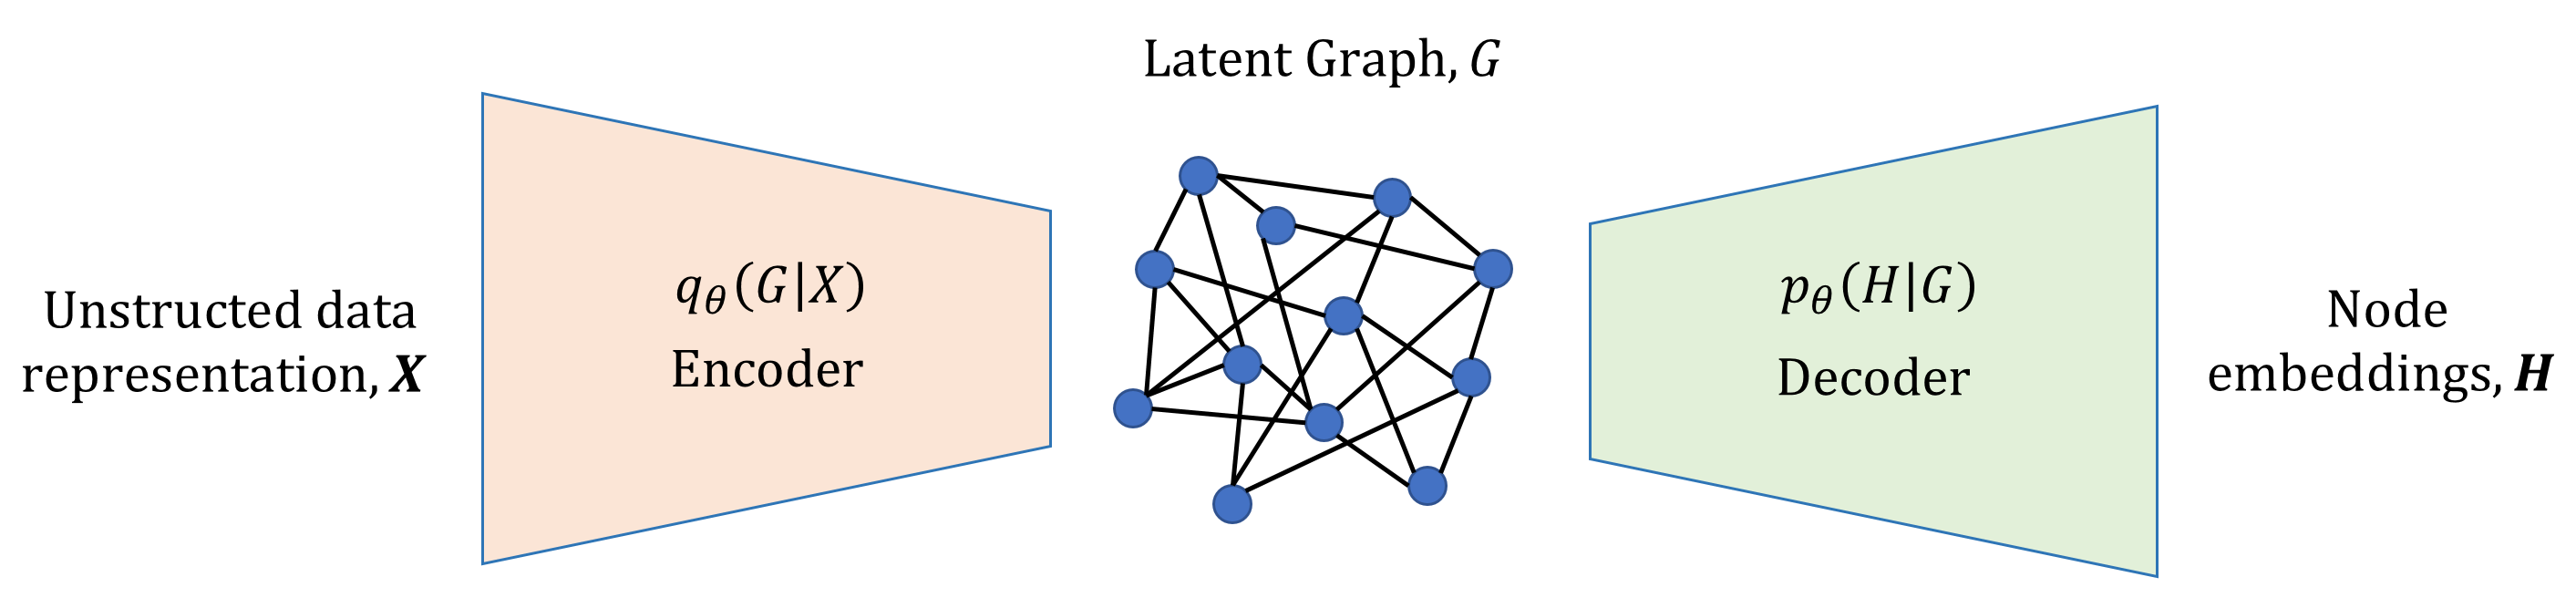
\includegraphics[width=\textwidth]{vae_figure.png}
		\caption{Representation of the variational autoencoder proposed. The input data to the encoder are the feature vectors of the data entities, and it is trained to output a latent graph, which is fed into the decoder. The decoder than learns the latent node embeddings from the inferred latent graph and its node features.\label{vae}}
	\end{figure}


	\subsection{Encoder}

	Given the requisite that our model should be able to take into account possible dependencies between the graph elements, the vanilla VAE encoder, as used by \textcite{KipfNRI2018} does not suit our needs. For us, the most interesting research direction is to leverage the idea of autoregressive generative models \citep{Li2018, You2018, Liao2019}, using one of the proposed approaches as the encoder of our VAE.

	Autoregressive models generate graphs sequentially, adding nodes and edges one at a time, taking into account the already generated elements. Thus, the creation of new elements in the graph explicitly considers the elements already in place, fulfilling the need of modelling the elements dependencies.

	Given the literature of autoregressive generative models \citep{Li2018, You2018, Liao2019}, one possible approach is to employ recurrent neural networks (RNN) to sequentially generate the graph elements, following the work of \textcite{You2018}.

	\textcite{You2018} proposed a model that uses two RNNs, one at the node-level and one at the edge-level. Each unit of the node-level RNN is responsible for creating a new node in the graph and it is associated with an entire edge-level RNN sequence.

	The edge-level RNN is a sequence having the same number of units as the number of nodes already created, with each unit outputting the probability of the existence of an edge between the node just created and the existing nodes in the graph. This probability is modeled as a Bernoulli distribution, and the result (existence or not of an edge) is fed into the next unit. After the last unit of the edge-level RNN has being processed, its hidden-state vector is send to the next unit of the node-level RNN.

	The autoregressive generative process is illustrated in Figure \ref{rnn1}. A visualization of what is happening in the graph adjacency matrix while the model is working can be seen in Figure \ref{rnn2}. The process ends when the node-level RNN has processed the features of all the entities of the input data and there is no more nodes to be created.

	\begin{figure}[hbtp]
	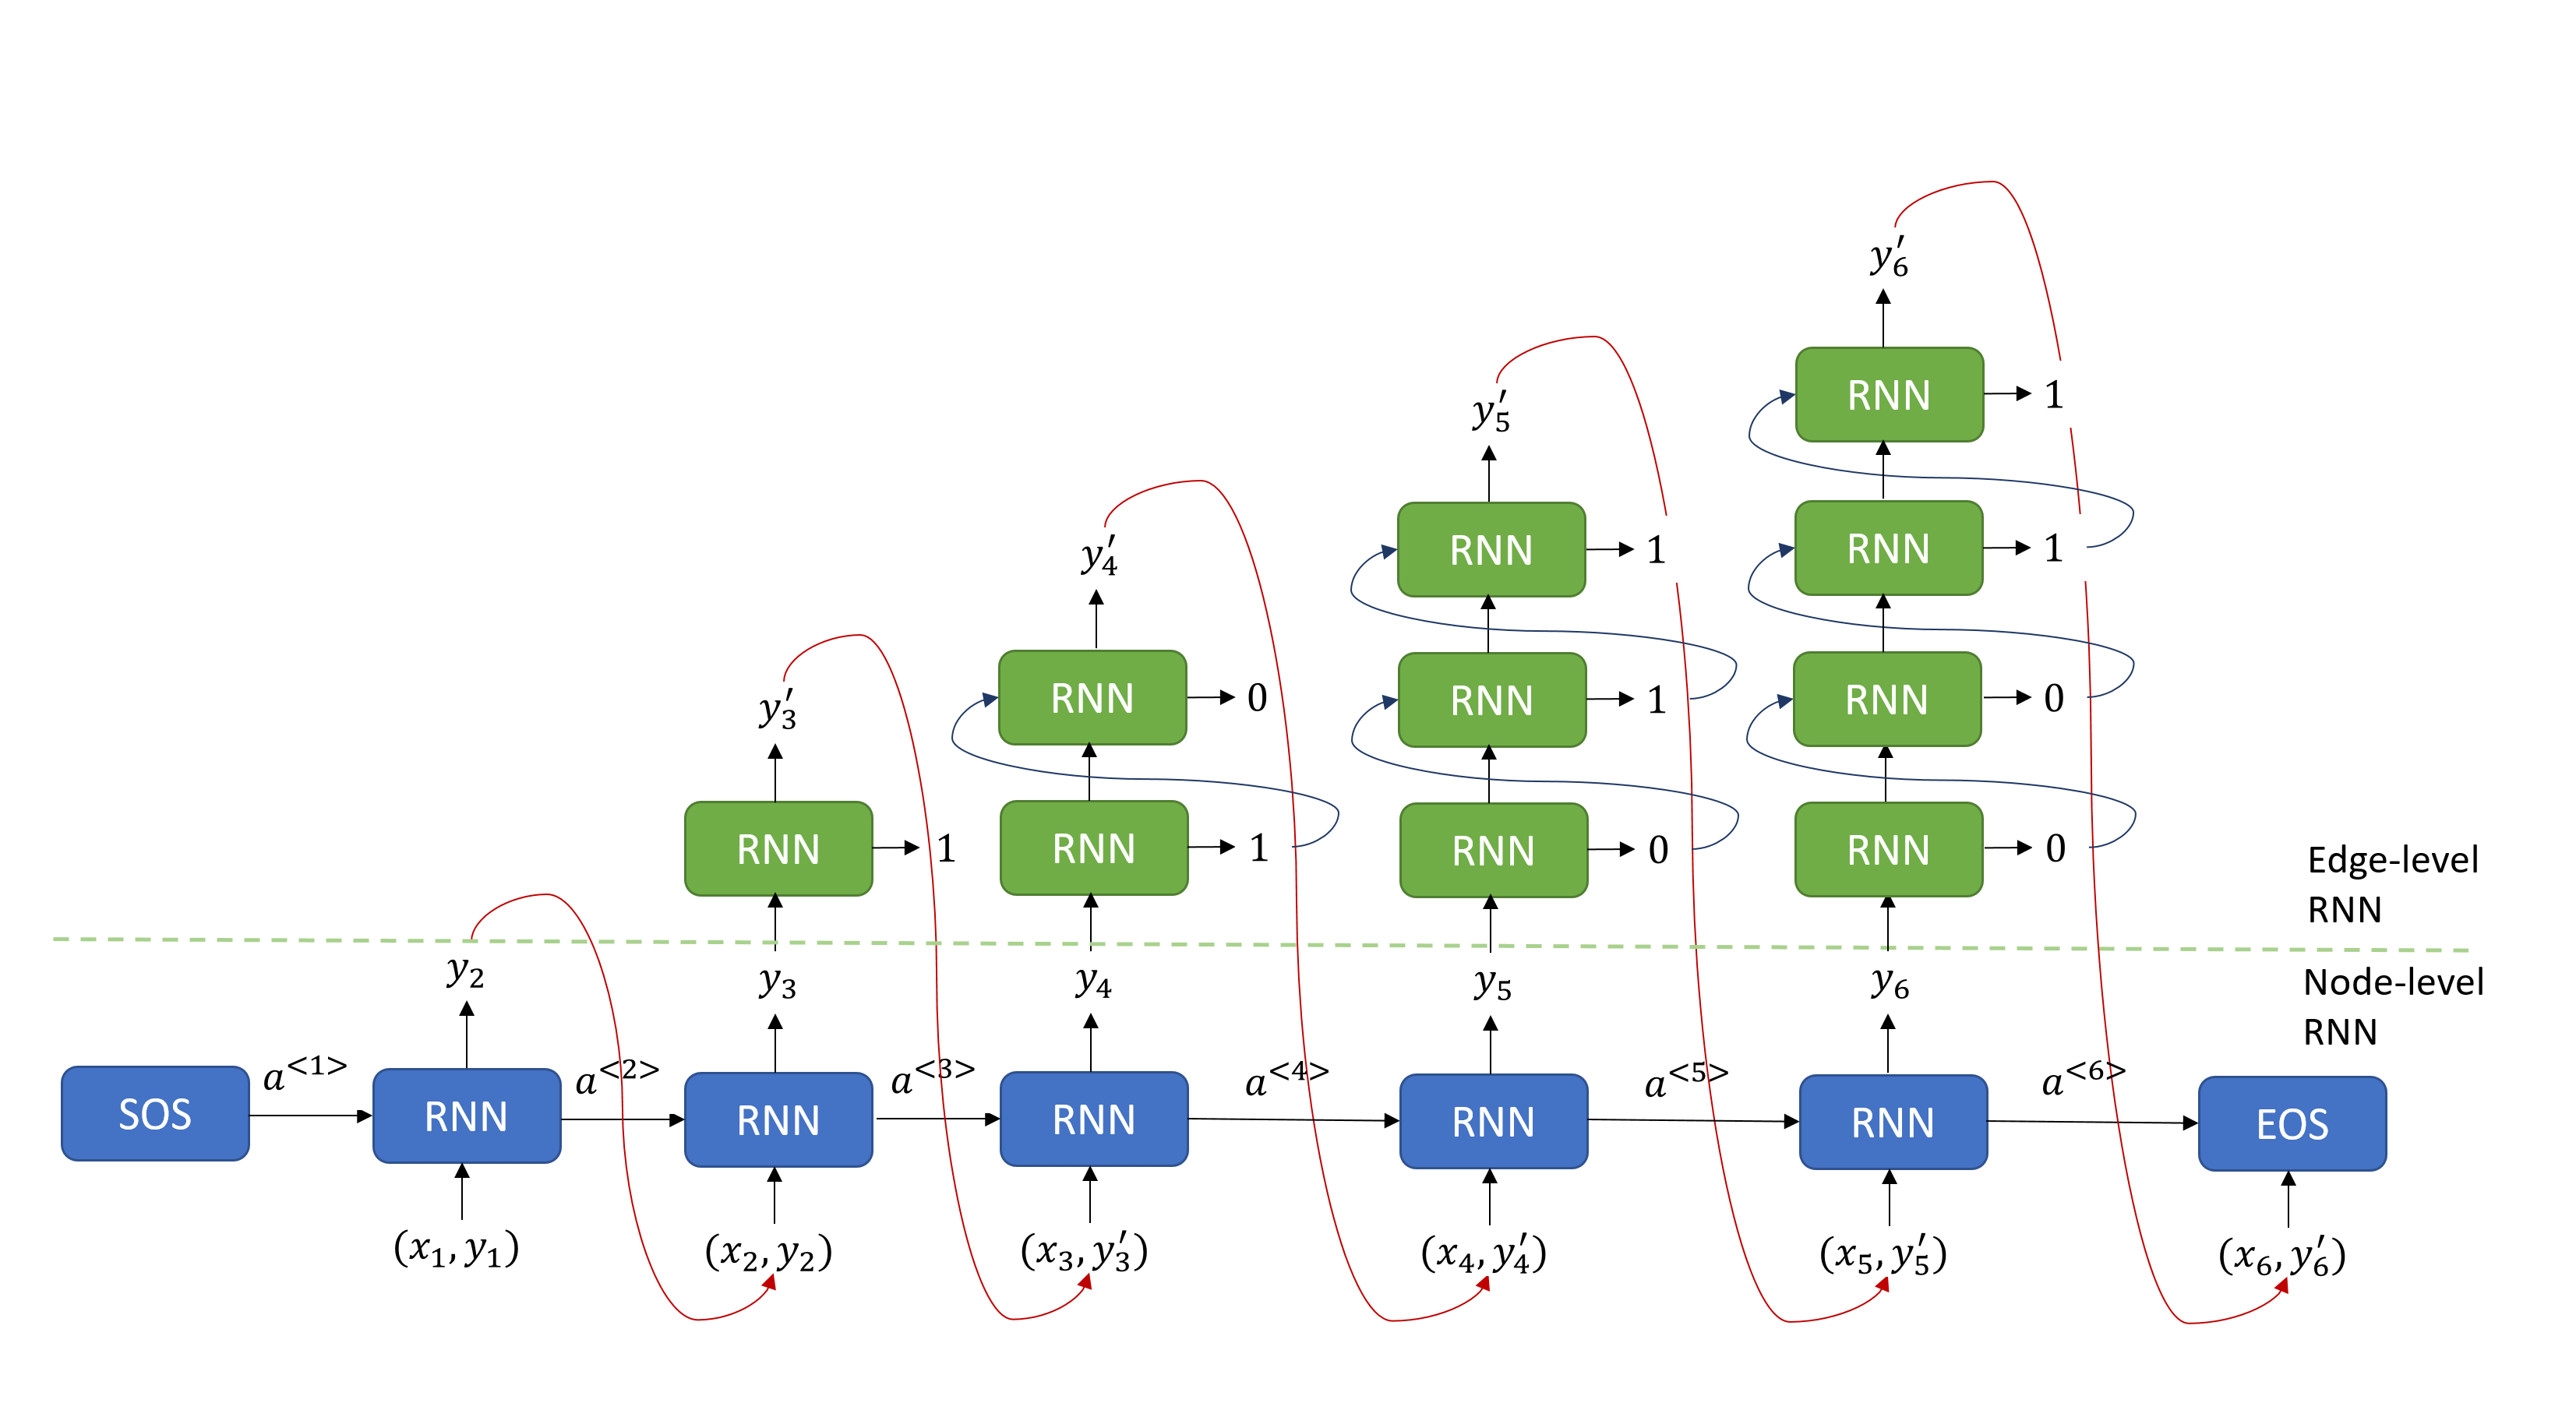
\includegraphics[width=\textwidth]{rnn.png}
	\caption{Autoregressive generative model, formed by a node-level RNN and an edge-level RNN. Each unit in the Node-level RNN receives as input features from the input data and the output of the previous Edge-level RNN, and its job is to create a new node in the latent graph. It also outputs a vector that is fed into the associated Edge-level RNN. The function of the Edge-level RNN is decide the presence or not of edges between the node just created the nodes that were created previously. \label{rnn1}}
	\end{figure}


	\begin{figure}[hbtp]
	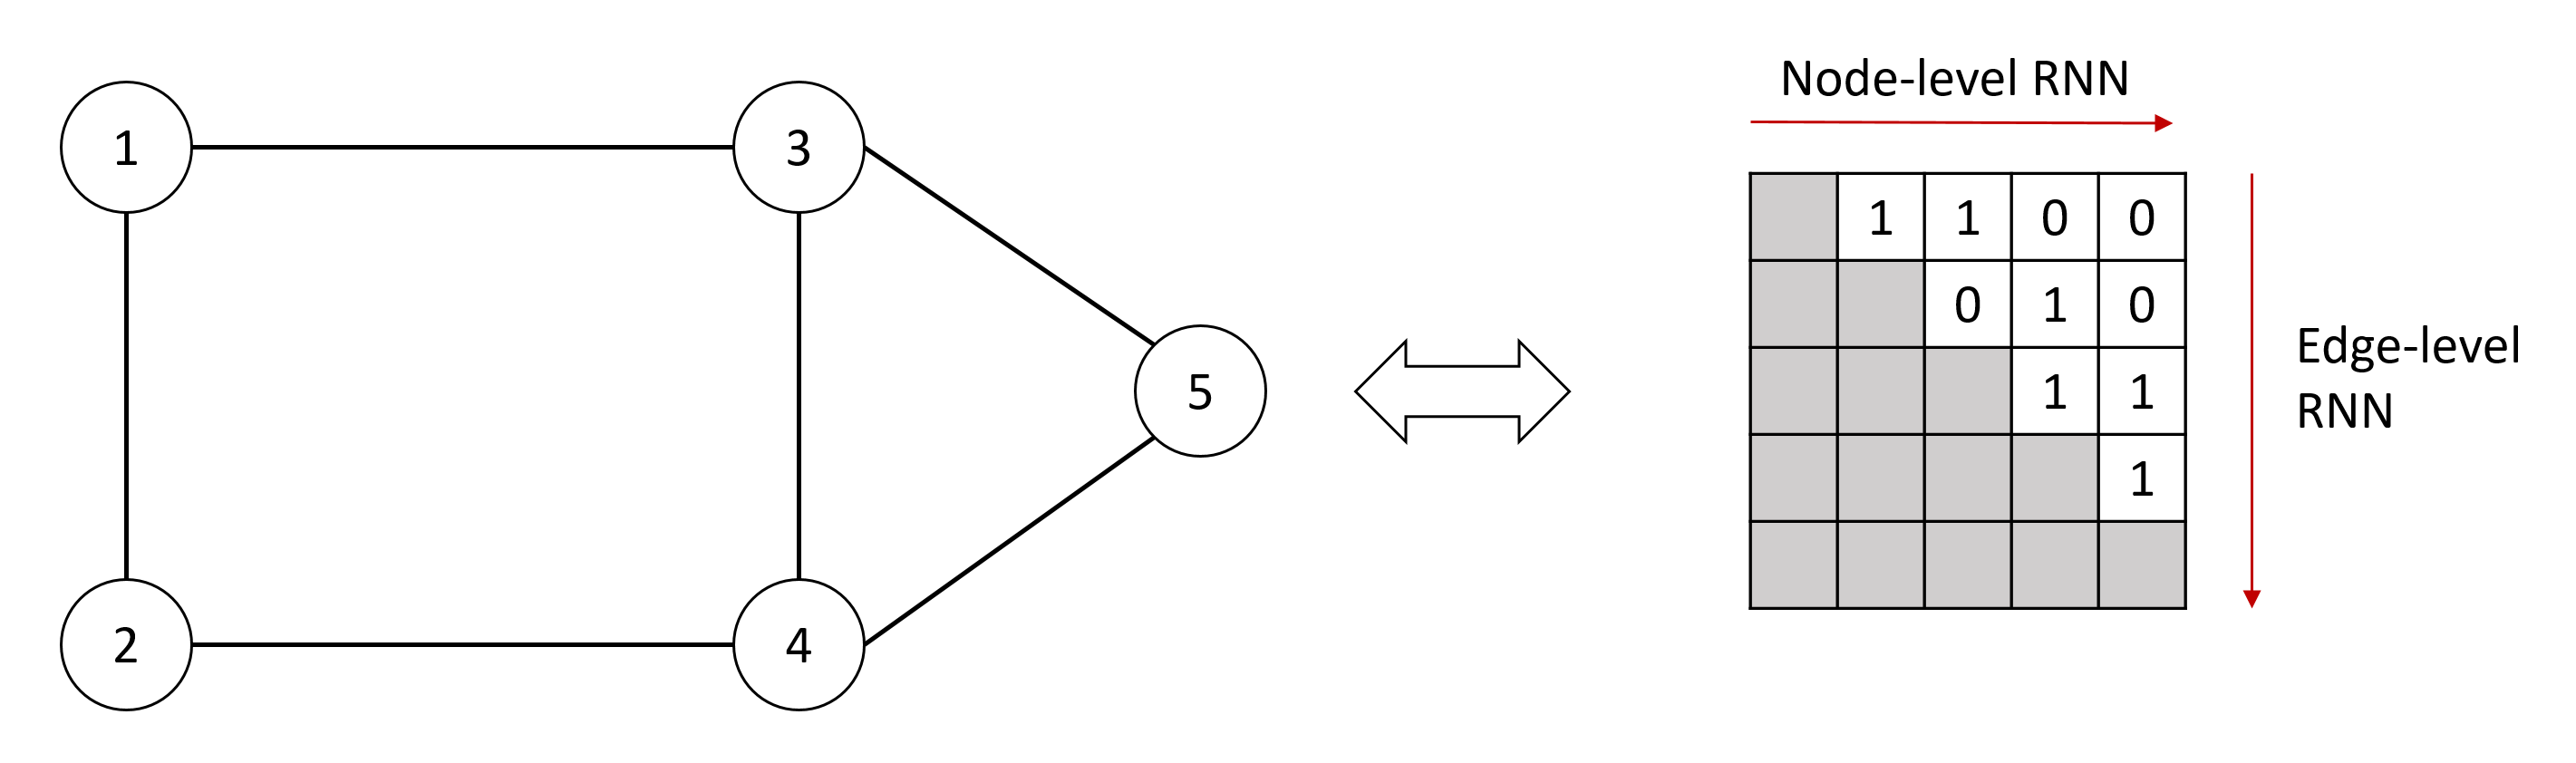
\includegraphics[width=\textwidth]{rnn_adj.png}
	\caption{Every unit in the node-level RNN means the creation of a new node in the latent graph, which is translated in the addition of a new column in the adjacency matrix. Similarly, every unit in the edge-level RNN decides the content of one element of that column, meaning deciding the presence or not of an edge between the nodes. \label{rnn2}}
	\end{figure}


	\subsection{Decoder}

	After the encoder has generated a latent graph from the unstructured data, we can use any GNN pipeline to process the graph and the node features as our decoder. Nevertheless, in order for our model to account for dynamic changes in the relationships between the data entities, a special type of GNN layer is needed. Inspired by the inner workings of the LSTM unit \citep{HochreiterandSchmidhuber1997}, we propose the use of a \emph{switch gate} attained to every edge in the network.

	The function of the \emph{switch gate} is to dynamically turn on or off the edges of the network, as the dynamics of the underlying data changes. For instance, in a soccer game the players may have an underlying graph representing each one of them and their relations, but as the ball passes along from player to player this graph may change, with some edges appearing or disappearing. The function of the \emph{switch gate} is to model these changes.

	The \emph{switch gate} receives the embeddings from the nodes connected by the edge, concatenates them and passes this input through a single layer perceptron and a sigmoid nonlinearity. The sigmoid nonlinearity has the objective to make it easy for the \emph{switch gate} to turn on or off any edge, just by making the value of its argument very positive or very negative.

	The mechanism works according to
	\begin{equation}
		\Gamma_{au}=\sigma\left(W_s(h^{(l-1)}_a, h^{(l-1)}_u) + b_s\right)\!\text{, }  u \in N(a)\text{,} \label{switch}
	\end{equation}
	where $\Gamma_{vu}$ is the \emph{switch coefficient} of the edge connecting nodes $v$ and $u$, $\sigma$ is the sigmoid nonlinearity, $W_s$ is a linear transformation, $h^{(l-1)}_v$ is the latent embedding of node $v$ in the layer $(l-1)$ of the GNN, $(\cdot,\cdot)$ denotes concatenation and $N(v)$ denotes the neighbors of node $v$.

	The application of the \emph{switch gate} in a GNN is similar to that of an attention coefficient, and can be used with most message passing GNN layers. It’s use is shown in
	\begin{equation}
	h^{(l)}_a = ReLU\left(W_{self}h^{(l-1)}_a+W_{neigh}\sum_{u \in N(a)}\Gamma_{au}h^{(l-1)}_u + b\right)\text{,} \label{gnn}
	\end{equation}
	where $W_{self}$ and $W_{neigh}$ are learnable weight matrices, $b$ is the learnable bias and $ReLU$ is the Rectified Linear Unit nonlinearity.

	The message passing of a GNN layer employing the \emph{switch gate} mechanism is illustrated on Figure \ref{gate}.

	\begin{figure}[hbtp]
	\centering 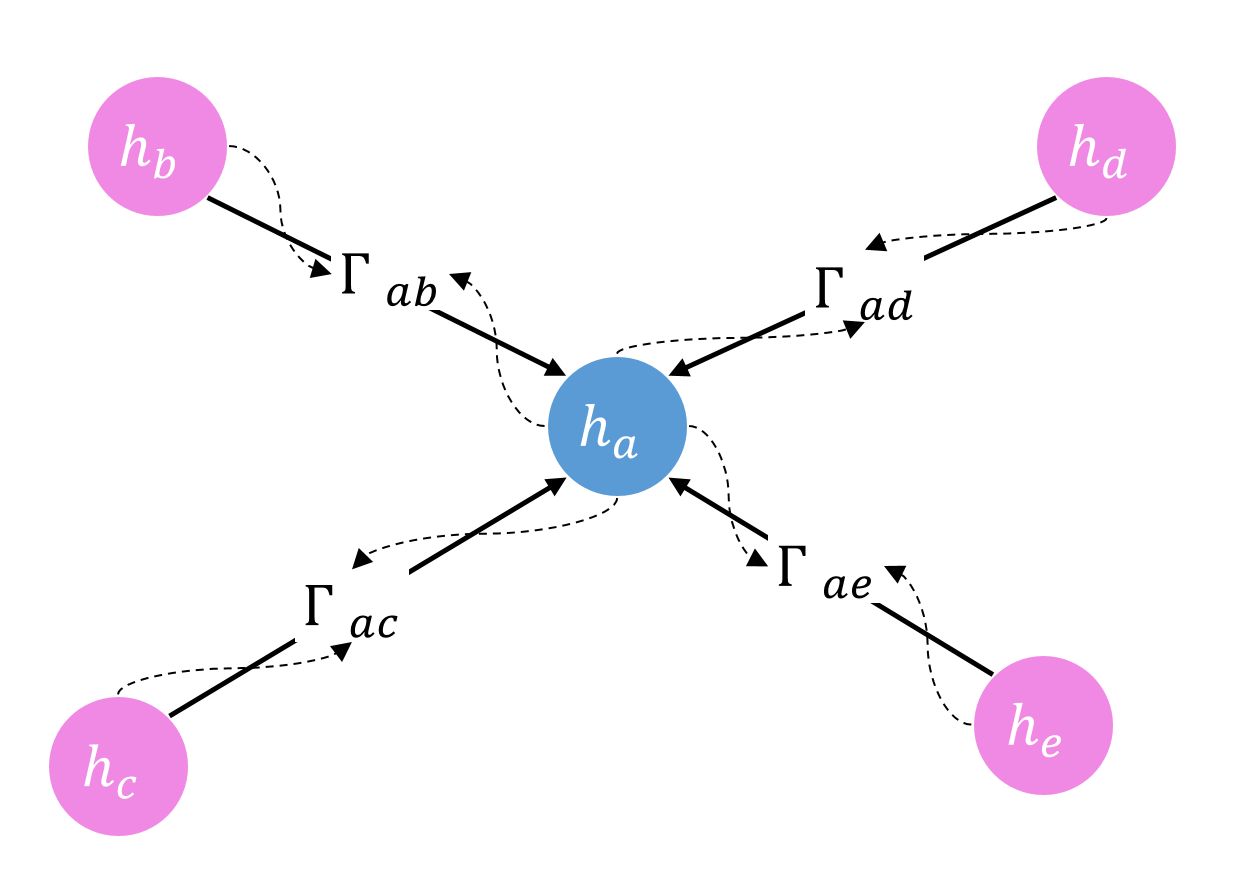
\includegraphics[scale=0.6]{gnn_w_gate.png}
	\caption{The \emph{switch gate} is calculated edge-wise, taking into account the embedding of the pair of nodes connected by the edge. Its functions is to turn on and off the edges of the network as the relations between the nodes change dynamically. \label{gate}}
	\end{figure}


	The decoder may employ a pipeline with a number of GNN layers using the \emph{switch gate} mechanism, as well as other common neural network layers and utilities, like dropout, batch normalization and shortcut connections. The best configurations will be evaluated in the course of the research.

	\section{Evaluation}
	\label{sec:Evaluation}

	In order to assess the fulfillment of the method requisites posed in Section 3, as well as its performance in prediction tasks, our model will undergo a three-part evaluation, being tested in five datasets in total. Each part of the evaluation has the purpose of assessing different aspects of the model.

	First, the model will be evaluated on its ability to simulate the behavior of physical multi-particle systems. Two simulated systems will be used for assessment: particles connected by springs and phase-coupled oscillators (Kuramoto model). The objective is to see how precisely the model can estimate the future state of these systems in comparison with our main benchmark, the NRI model \citep{KipfNRI2018}.

	Secondly, we will use the CMU Motion Capture Database \citep{CMU2003}, a large collection of motion recording performed by human subjects. We will evaluate our model in the walking motion data. This part of the evaluation is most interesting because \textcite{KipfNRI2018} has shown that the latent graph for this task is dynamic, changing as the skeleton performs the left and right steps. We use this dataset to compare our model with the NRI model and to evaluate the performance of our \emph{switch gate}.

	The setting for training and testing of the model in parts 1 and 2 of the evaluation are shown in Figure \ref{eval1}.

	Lastly, we evaluate our model in the Cora and Citeseer citation networks. The graphs from these datasets, though small, are much larger in number of entities than the data from the parts 1 and 2 of the evaluation, having 2,708 and 3,327 nodes respectively. The objective here is threefold: Firstly, we want to observe how well our encoder is able to scale to thousands of nodes, having to perform backward propagation for a long chain of RNN units (one for each node). Secondly, we want to investigate the benefits (if any) of inferring the latent graph from already structured data, comparing its performance with the performance of the \emph{explicit} or \emph{natural graph} in prediction tasks. This evaluation setting is illustrated on Figure \ref{eval3_1}. Lastly, we also want to evaluate the use of the latent graph as a mean of data augmentation, working \emph{together} with the \emph{explicit} graph, as shown in Figure \ref{eval3_2}.

	Our model will not have access to the Cora and Citeseer graphs, having to compute its own latent graph solely from the node features.

	\begin{figure}[hbtp]
		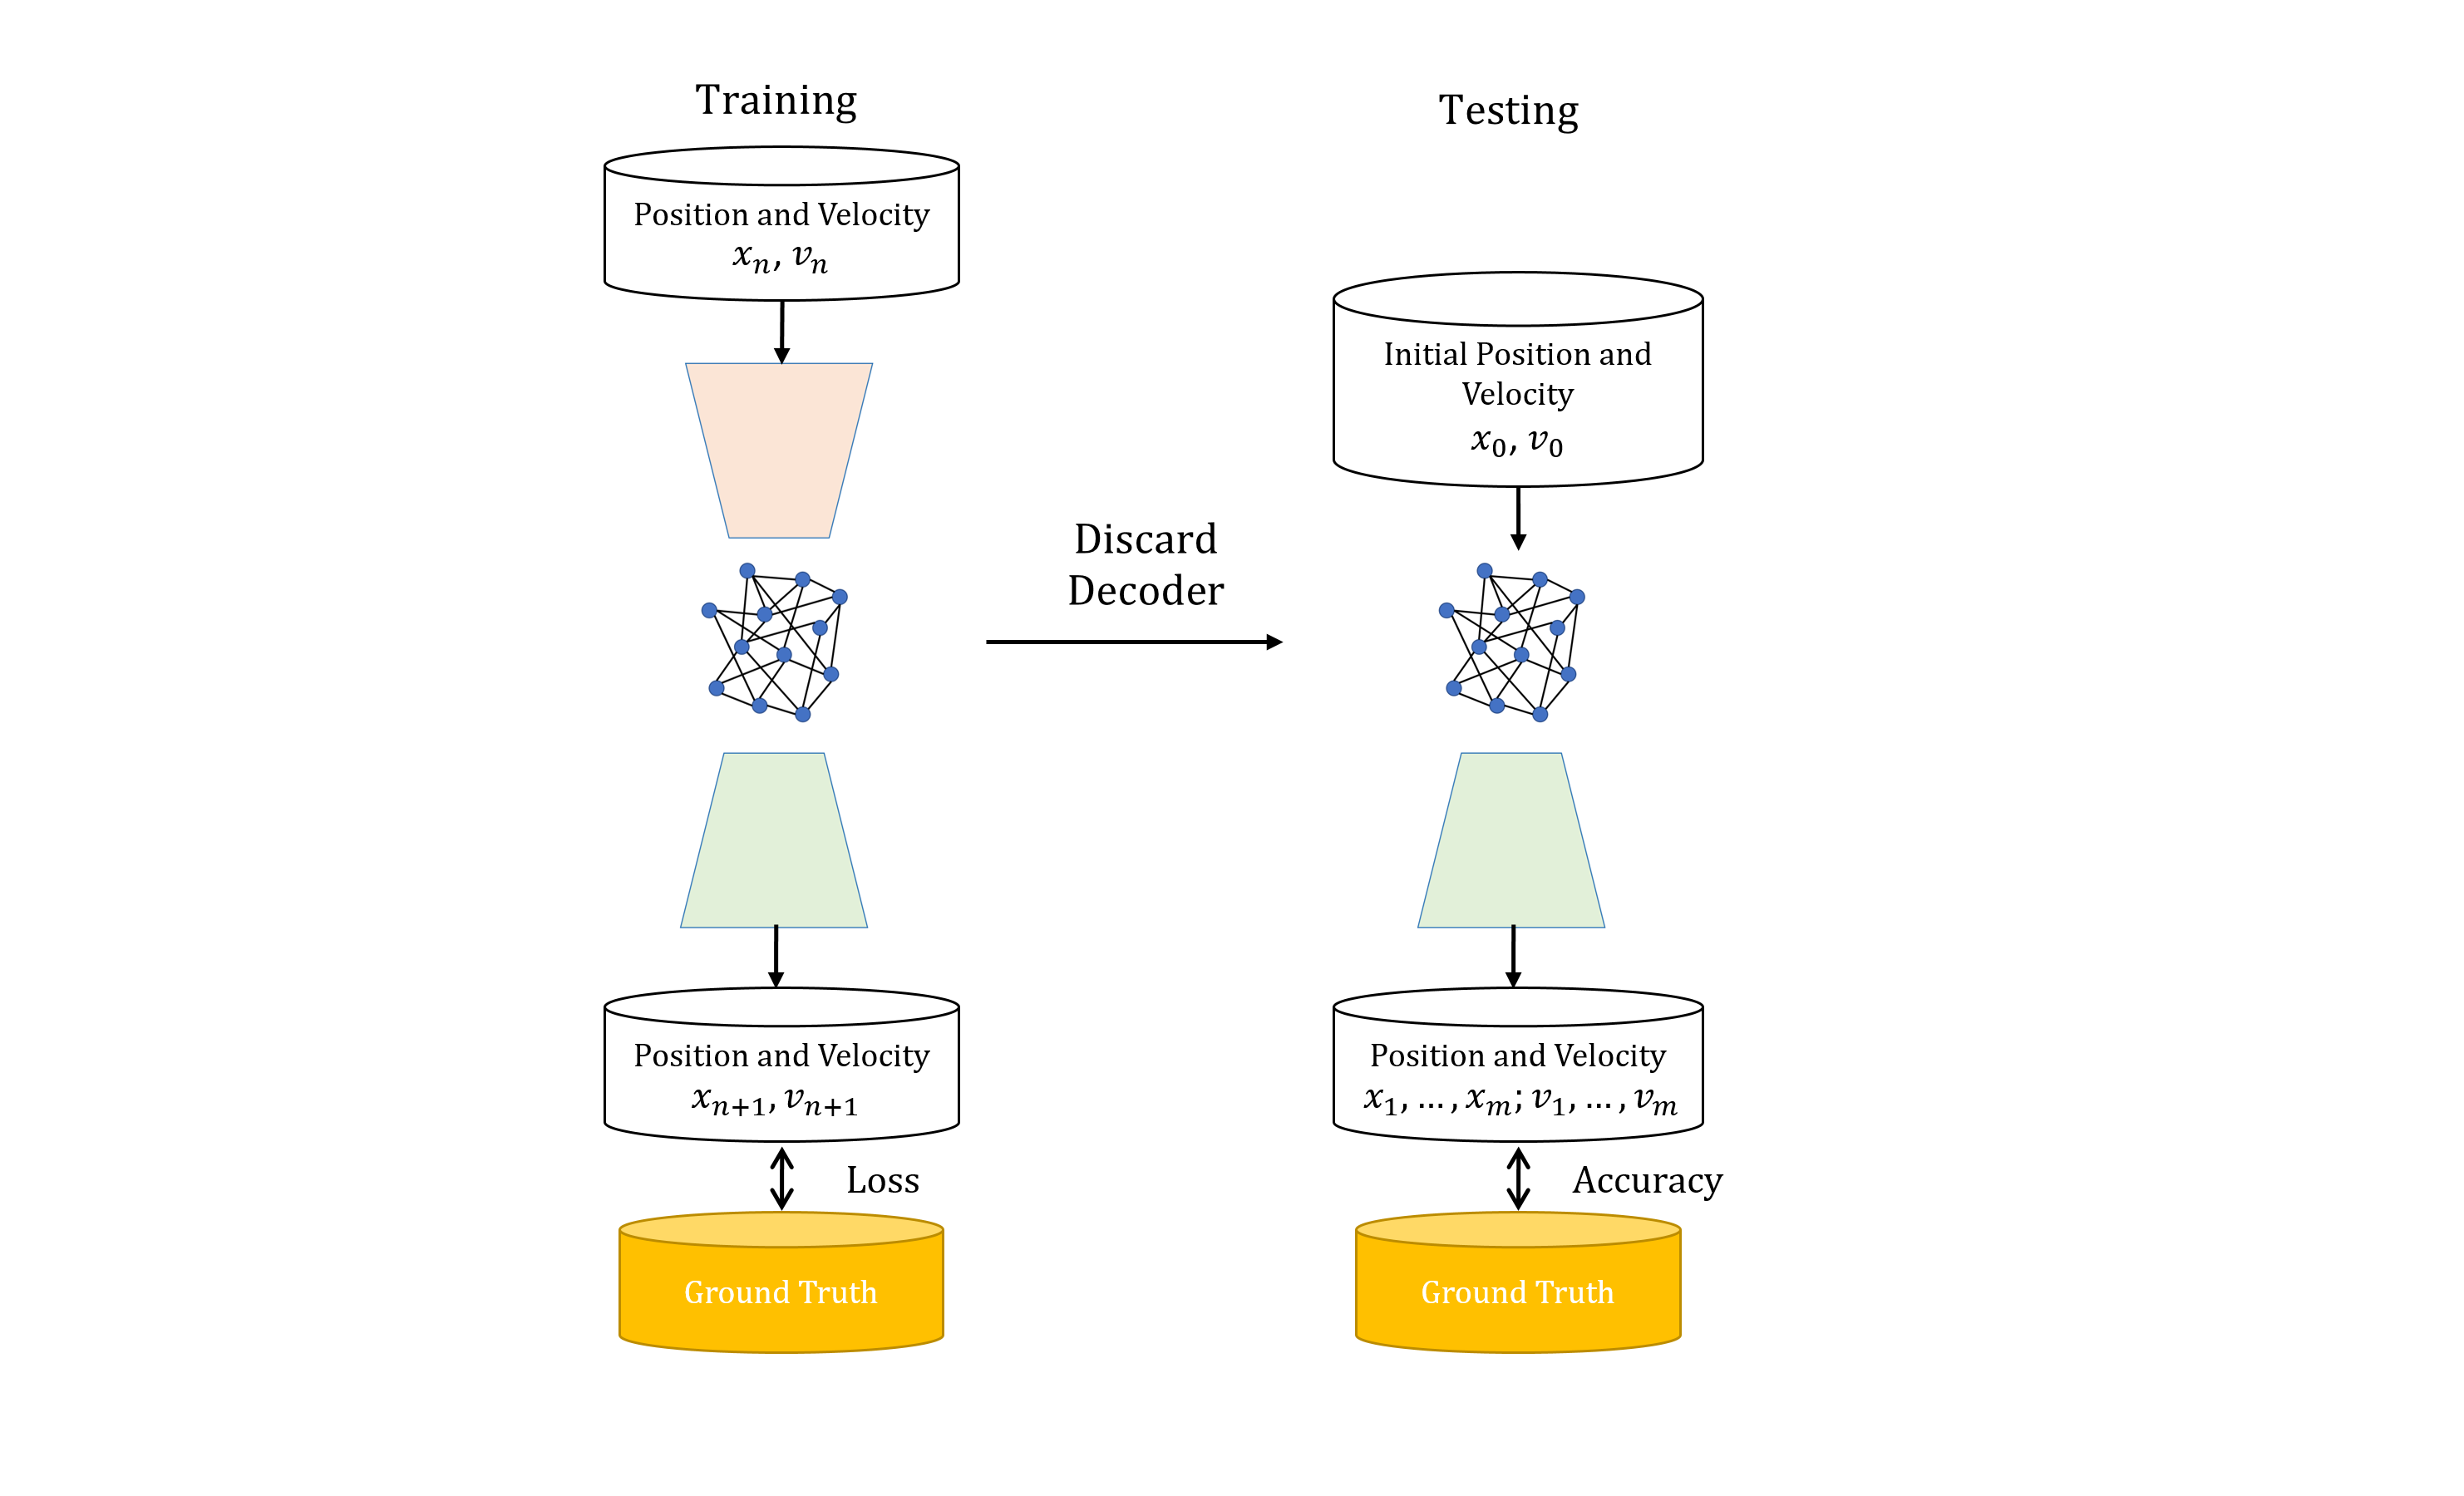
\includegraphics[width=\textwidth]{eval_part1_2.png}
		\caption{Setting for the training and evaluation of the model when predicting the future state of physical systems and the walking motion data. The encoder and decoder will be trained jointly, receiving the position and velocity of the entities at time n, and predicting the position and velocity for time n+1. After the system is trained, the encoder has already inferred the latent graph for the underlying data, and thus can be discarded. At test time we use only the latent graph and the decoder, that receives an initial position and velocity and predicts the future trajectories of the system. \label{eval1}}
	\end{figure}

	\begin{figure}[hbtp]
		\centering 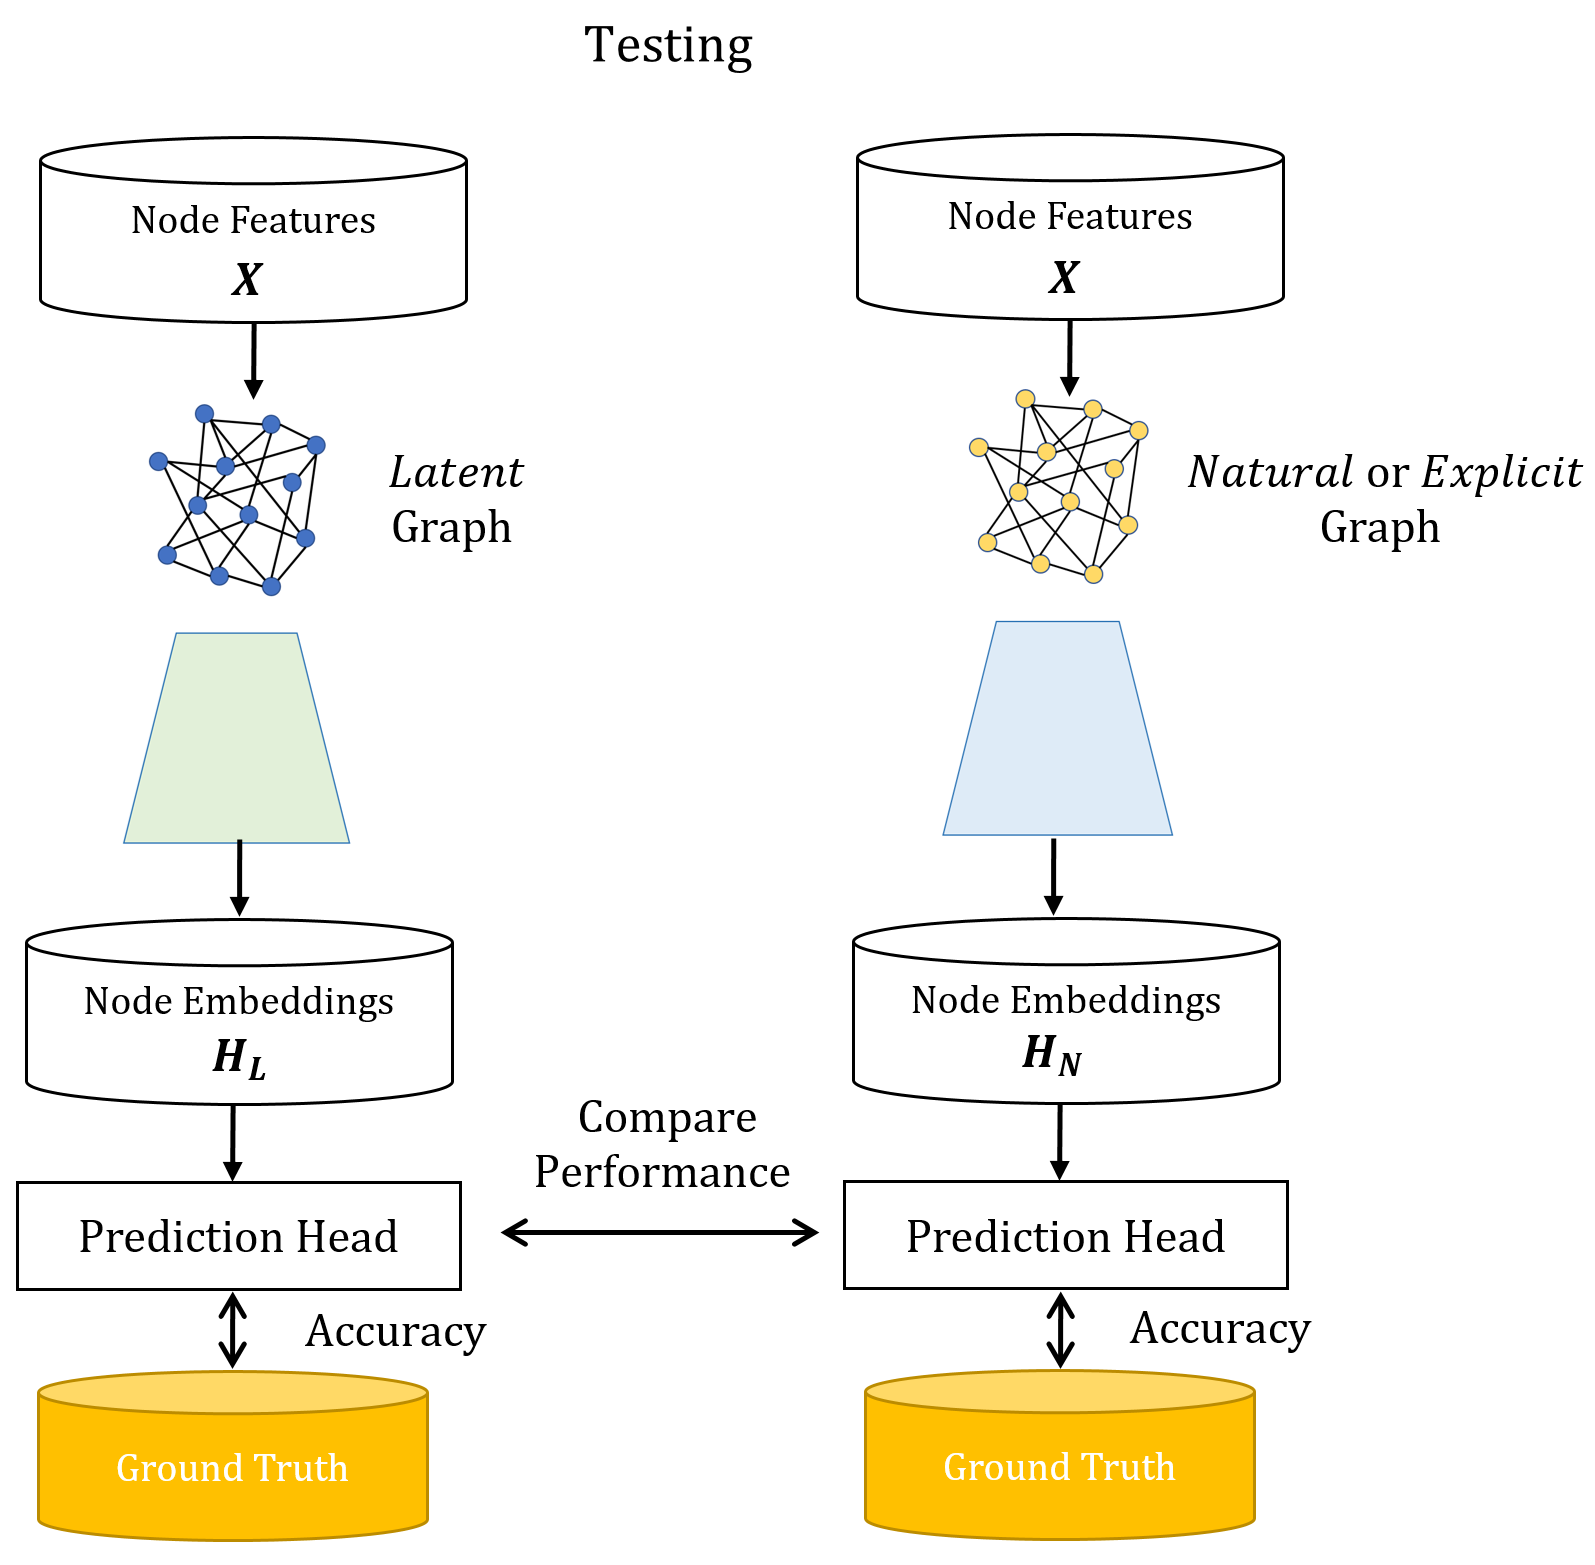
\includegraphics[scale=0.4]{eval_part3_1.png}
		\caption{After our model is trained, we use the latent graph to predict the node classes for the network. In parallel, the same predictions are performed using the \emph{natural} or \emph{explicit} graph, and the accuracies of both pipelines are then be compared. \label{eval3_1}}
	\end{figure}

	\begin{figure}[hbtp]
		\centering 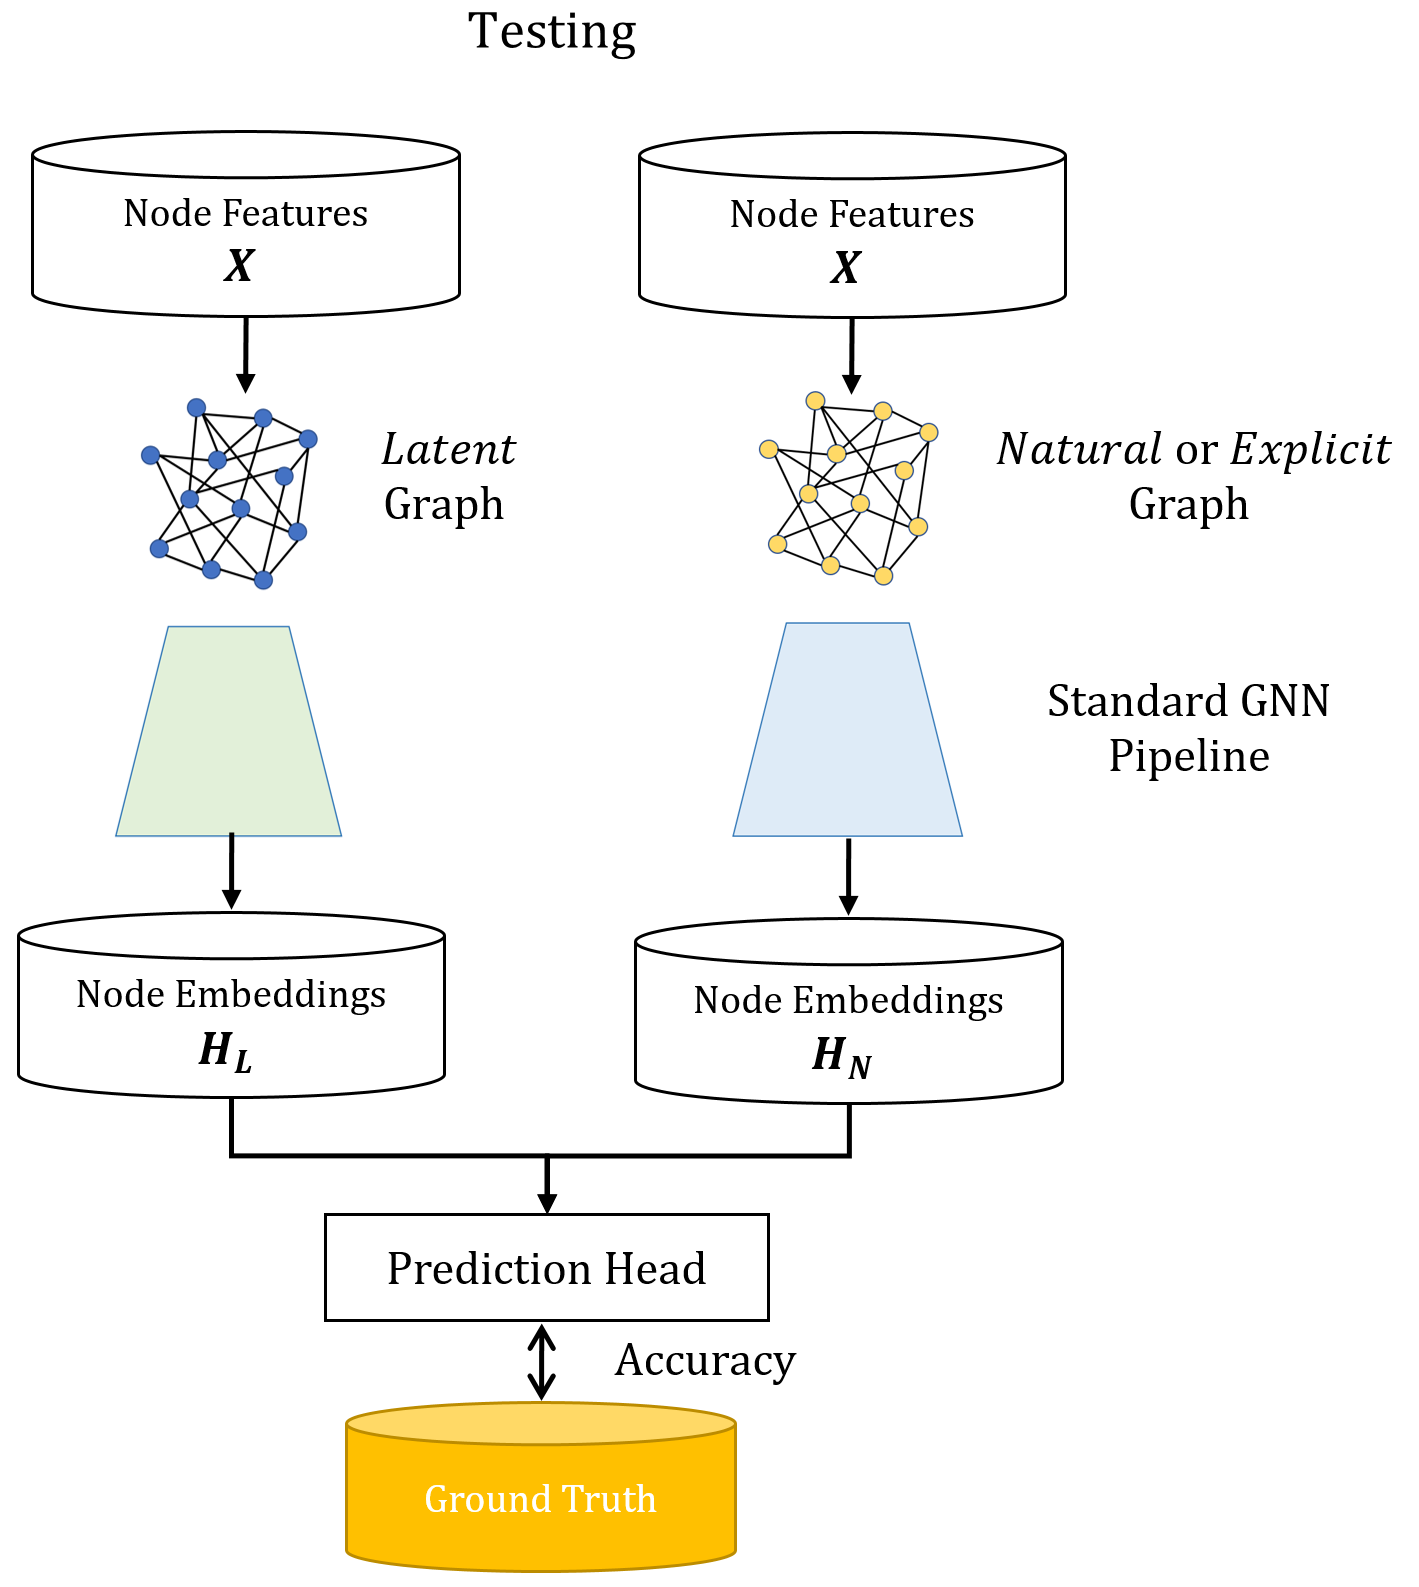
\includegraphics[scale=0.4]{eval_part3_2.png}
		\caption{The model will be used as a method of data augmentation, with the node embeddings generated from the latent graph and from the \emph{explicit} graph being combined before making the predictions. \label{eval3_2}}
	\end{figure}

	\section{Activities and Schedule}
	\label{sec:Activities_and_schedule}

	The research has duration of approximately 2 years, with proposed deadline in December of 2023. 

	The main activities that will be performed in the duration of the research are:

	\begin{itemize}
	\item[a)] Review of the literature on the main topics of the research: inference of latent graph from unstructured data, machine learning on graphs and generative methods for graphs;
	\item[b)] Based on the gaps observed in the state of the art techniques, a new method will be proposed for the inference of latent graphs from unstructured data, along the lines described in this document;
	\item[c)] Perform evaluation and assessments of the proposed models and possible variations of it, as described in Section 5, comparing them with the state of the art techniques.
	\item[d)] Write an annual report about the research developments in December 2022;
	\item[e)] Publish a scientific paper with the main findings of the research by December 2023;
	\item[f)] Make the implementation of the method available in public domain; and
	\item[g)] Perform a 6-month research internship abroad as a visiting scholar (FAPESP BEPE scholarship).
	\end{itemize}

	The proponent started the master's degree program in August of 2021, and since the aforementioned date has been working on the review of the literature on the main topics of the research, in order to build the proposal presented in this document.

	The proposed activities and the estimated research schedule can be seen in a Gantt chart on Figure \ref{plan}.

	\begin{figure}[hbtp]
		%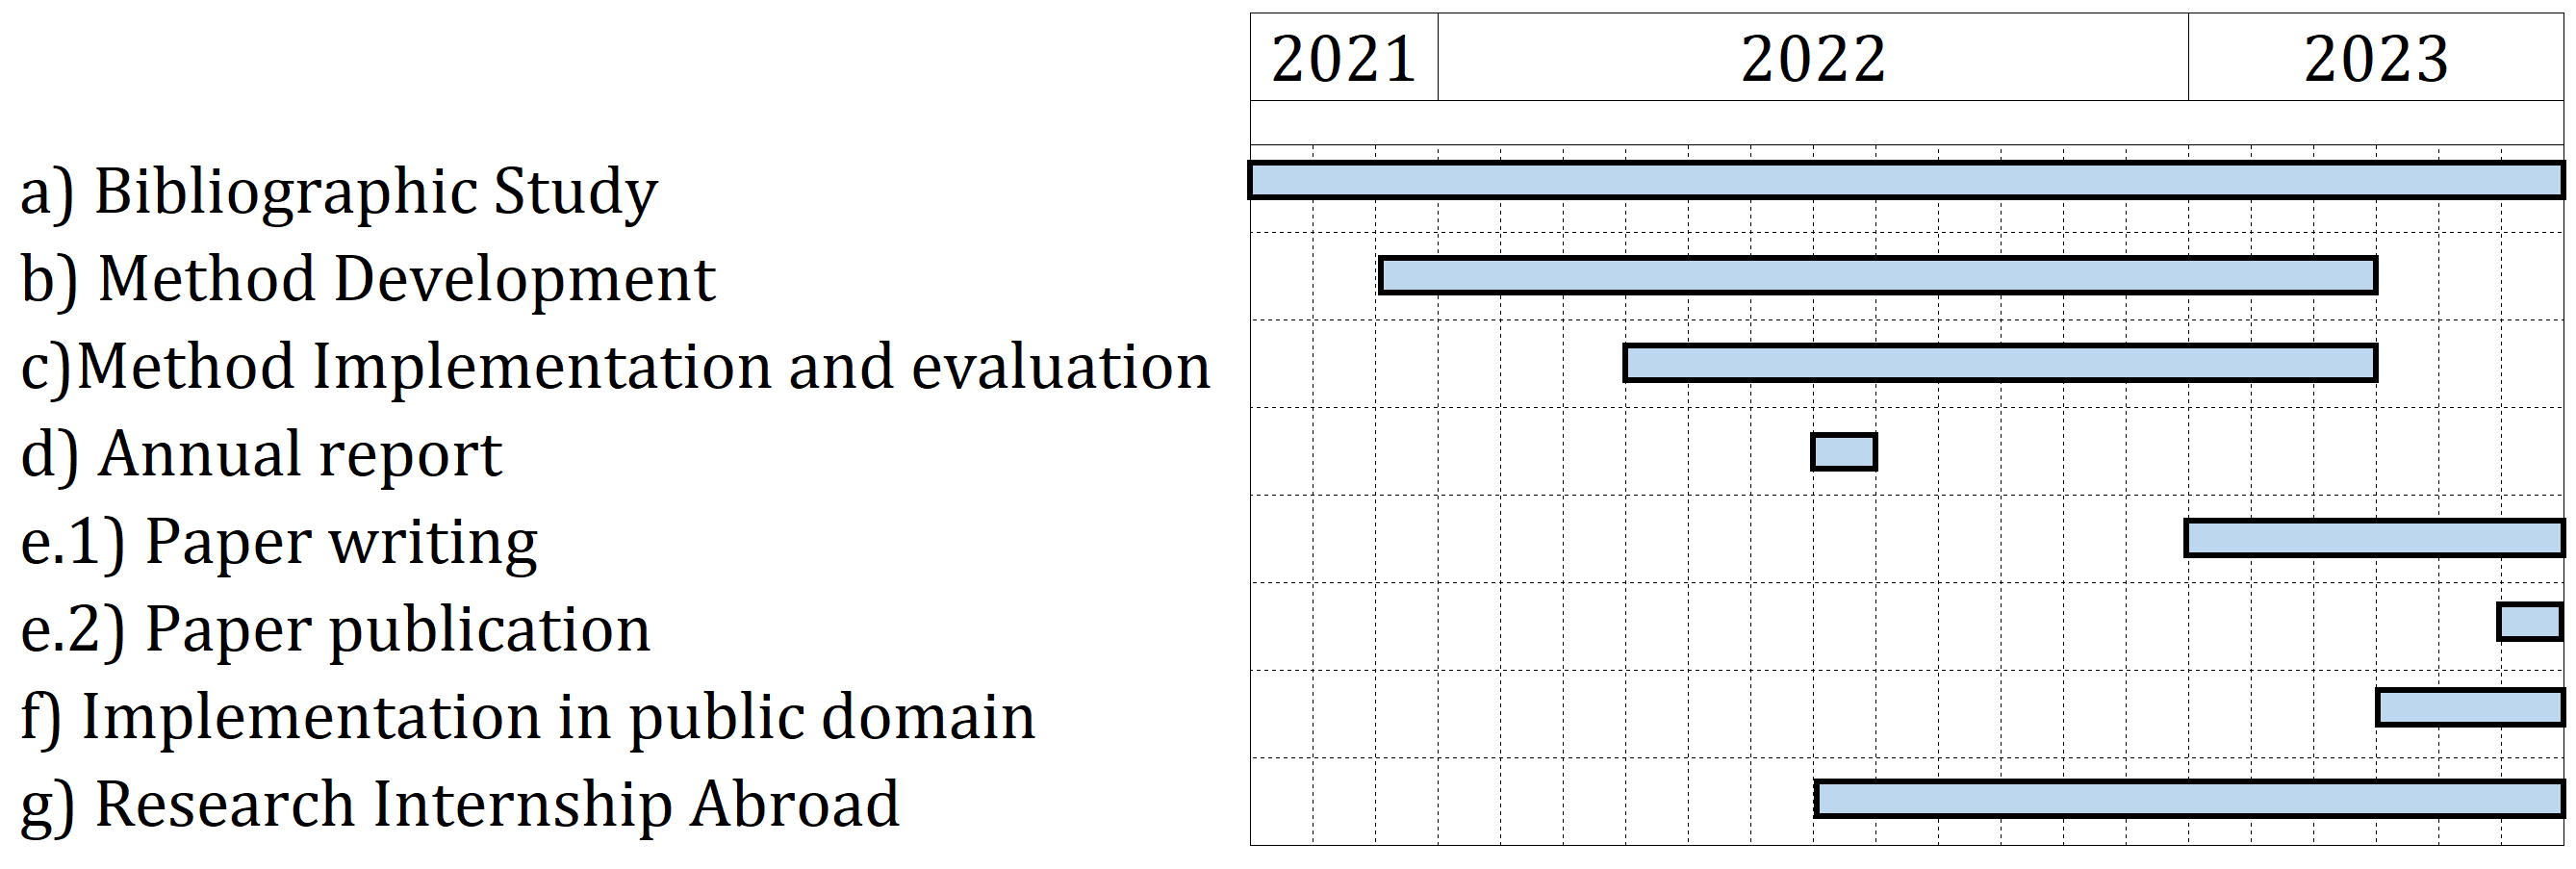
\includegraphics[width=\textwidth]{plan_v2.png}
		\centering 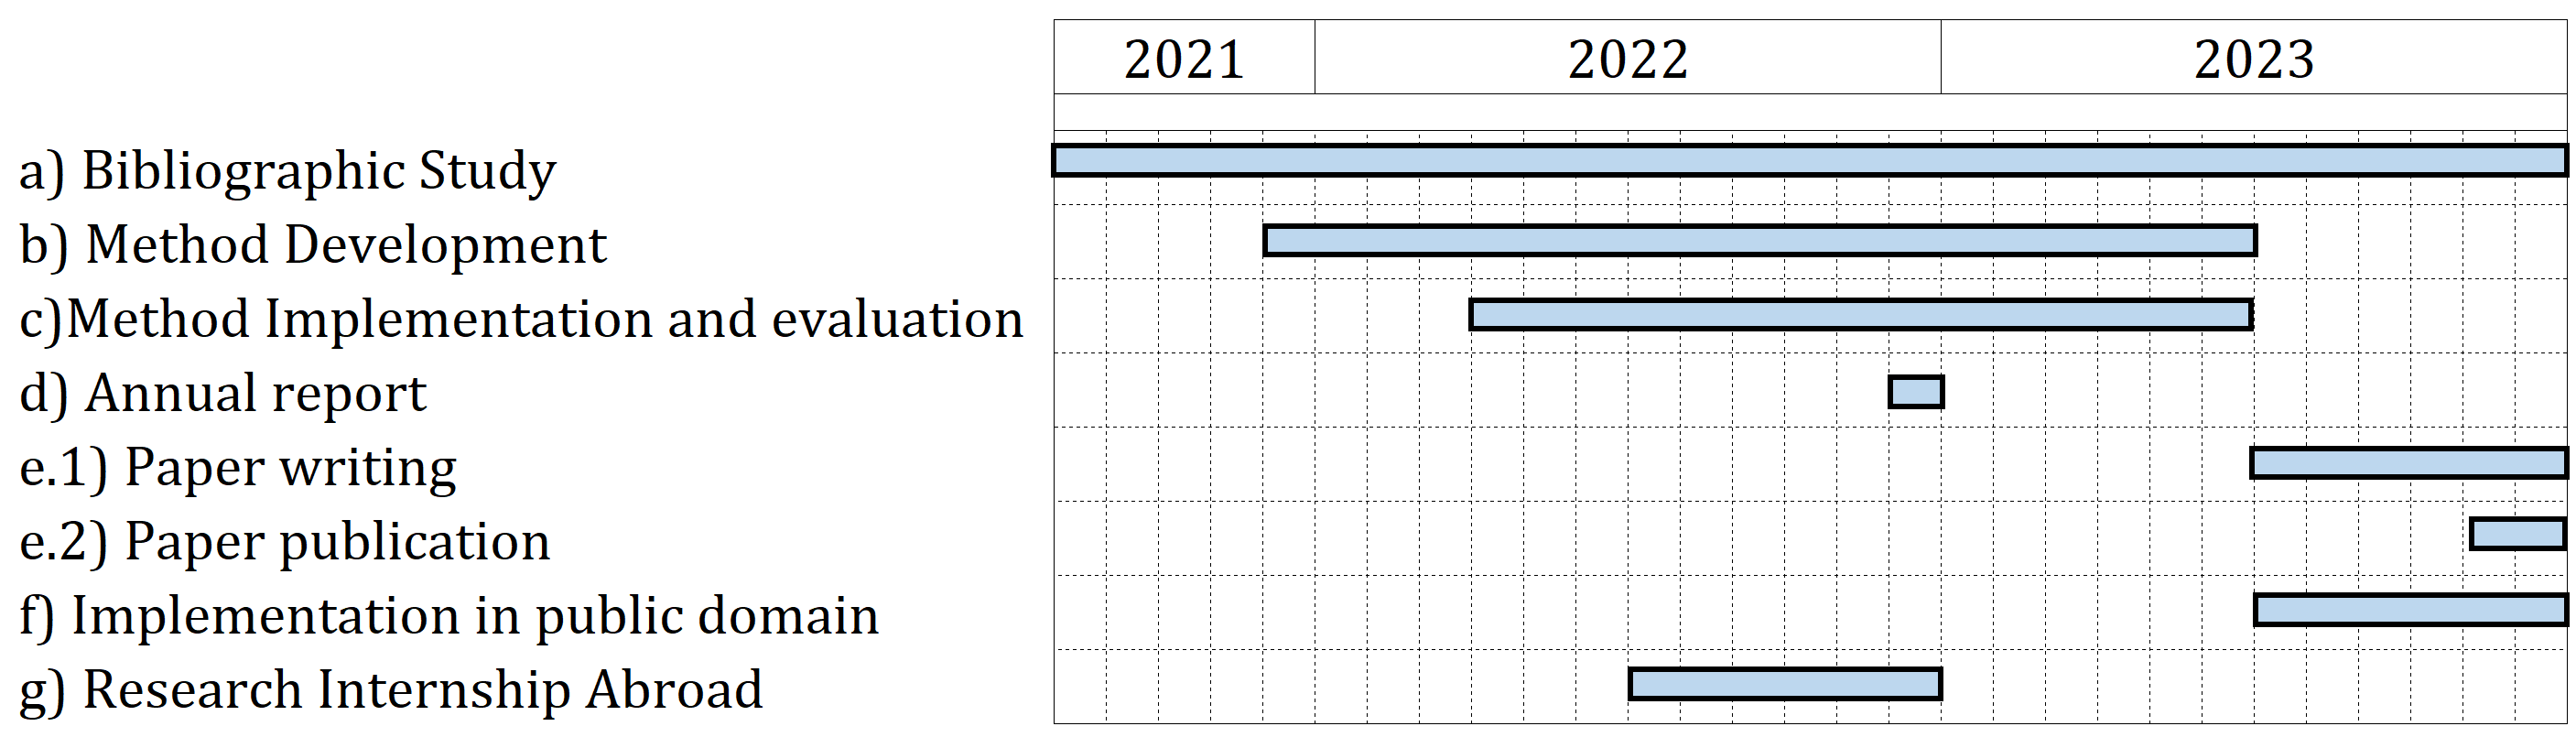
\includegraphics[scale=0.40]{plan_v3.png}
		\caption{Proposed activities and estimated research schedule. \label{plan}}
	\end{figure}

	\printbibliography

\end{document}
